\heading{理论力学-21秋-期末}

\begin{question}[旋转轻杆的角动量]
一根长为 $2l$ 的轻杆两端分别固定有质量为 $m$ 和 $2m$ 的两个质点。轻杆与竖直方向的夹角为 $\alpha$，其中点固定，并绕竖直轴以角速度 $\omega$ 匀速转动。建立合适的坐标系，求：
\begin{enumerate}
  \item 系统的角动量；
  \item 作用在 $O$ 点的力矩。
\end{enumerate}

\begin{solution}
设从 $O$ 指向质量为 $m$ 的质点的单位矢量为
\[
  \boldsymbol n=\sin\alpha\,\boldsymbol e_r+
  \cos\alpha\,\boldsymbol e_z,
\]
则两质点的位置可取为
\[
  \boldsymbol r_1=l\boldsymbol n,
  \qquad
  \boldsymbol r_2=-l\boldsymbol n.
\]
系统以角速度 $\boldsymbol\omega=\omega\boldsymbol e_z$ 转动。对任一质点，
\[
  \boldsymbol r\times m(\boldsymbol\omega\times\boldsymbol r)
  =m l^2\omega(\boldsymbol e_z-\cos\alpha\,\boldsymbol n).
\]
因此系统角动量为
\[
  \boxed{\boldsymbol L=3ml^2\omega
  \left(\sin^2\alpha\,\boldsymbol e_z
  -\sin\alpha\cos\alpha\,\boldsymbol e_r\right)}.
\]
由于 $\boldsymbol e_r$ 随杆一起绕竖直轴转动，
\[
  \frac{\dd\boldsymbol e_r}{\dd t}=\omega\boldsymbol e_\varphi .
\]
故合外力矩为
\[
  \boxed{\boldsymbol M=\frac{\dd\boldsymbol L}{\dd t}
  =-3ml^2\omega^2\sin\alpha\cos\alpha\,\boldsymbol e_\varphi}.
\]
若要求支点 $O$ 对系统提供的力矩，还需扣除重力矩。按上述质量标号，重力矩为
\[
  \boldsymbol M_g=-mgl\sin\alpha\,\boldsymbol e_\varphi,
\]
所以
\[
  \boldsymbol M_O=\boldsymbol M-\boldsymbol M_g
  =m l\sin\alpha\left(g-3l\omega^2\cos\alpha\right)\boldsymbol e_\varphi .
\]


\medskip
\textbf{推导核查：}上式也可从惯量张量理解。由于两个质点到 $O$ 的距离均为 $l$，但质量和为 $3m$，系统相对于通过 $O$ 且垂直轻杆方向的转动惯量为 $3ml^2$，相对于轻杆自身的转动惯量为零。把角速度分解为
\[
  \boldsymbol\omega=\omega\cos\alpha\,\boldsymbol n
  +\omega\left(\boldsymbol e_z-\cos\alpha\,\boldsymbol n\right),
\]
沿杆分量不贡献角动量，垂直杆分量才贡献角动量，因此
\[
  \boldsymbol L=3ml^2\omega\left(\boldsymbol e_z-\cos\alpha\,\boldsymbol n\right).
\]
代入 $\boldsymbol n=\sin\alpha\boldsymbol e_r+\cos\alpha\boldsymbol e_z$ 即得前面的结果。求力矩时要注意 $\boldsymbol L$ 的大小不变，但其水平分量方向随时间转动，因此 $\dd\boldsymbol L/\dd t$ 不为零。
\end{solution}
\end{question}

\begin{question}[击打均匀球后的纯滚动]
一个半径为 $R$ 的均匀球放在粗糙水平地面上，球与地面的摩擦系数为 $\mu$。现沿水平方向击打球面上一点，该点距球心的竖直高度为 $\frac{6}{7}R$。击打后球的质心速度大小为 $v_0$。求球进入纯滚动状态时的平动速度。

\begin{solution}
取球向右平动为正，并取顺时针角速度为正。设击打冲量为 $J$，则
\[
  mv_0=J.
\]
击打点相对球心的力臂为 $6R/7$，均匀球的转动惯量为
\[
  I=\frac25mR^2.
\]
击打后初始角速度为
\[
  \omega_0=\frac{J(6R/7)}{I}
  =\frac{15}{7}\frac{v_0}{R}.
\]
球在滑动到纯滚动的过程中，关于地面接触点的角动量守恒。初始角动量为
\[
  L_i=mRv_0+I\omega_0
  =mRv_0+\frac25mR^2\frac{15v_0}{7R}
  =\frac{13}{7}mRv_0 .
\]
纯滚动时 $\omega=v/R$，故
\[
  L_f=mRv+I\frac{v}{R}
      =\frac75mRv .
\]
令 $L_i=L_f$，得
\[
  \boxed{v=\frac{65}{49}v_0}.
\]
结果大于 $v_0$，说明滑动摩擦在此过程中增加了质心平动速度，同时减少了过大的初始转动。


\medskip
\textbf{关键步骤：}也可显式引入滑动摩擦冲量 $J_f$ 来看符号。击打后底点速度为
\[
  v_0-R\omega_0=v_0-\frac{15}{7}v_0=-\frac87v_0,
\]
即底点相对地面向左滑动，所以地面对球的摩擦力向右。滑动阶段有
\[
  m(v-v_0)=J_f,
  \qquad
  I(\omega-\omega_0)=-RJ_f,
\]
负号表示向右摩擦使顺时针角速度减小。纯滚动条件为 $v=R\omega$。把 $I=2mR^2/5$ 代入三式，可解得同样的
\[
  v=\frac{65}{49}v_0.
\]
摩擦系数 $\mu$ 只影响达到纯滚动所需时间；只要有足够粗糙接触使滑动最终停止，最终速度与 $\mu$ 无关。


\medskip
若需要判断纯滚动前是否一直滑动，可由底点相对速度
\[
  u=v-R\omega
\]
写出
\[
  \dot u=\dot v-R\dot\omega=\frac{\mu mg}{m}-R\left(-\frac{\mu mgR}{I}\right)
  =\mu g\left(1+\frac{mR^2}{I}\right)>0,
\]
其中取底点初速度 $u_0=-8v_0/7<0$。因此 $u$ 会单调增至零，确实能达到纯滚动。这个过程还说明摩擦力方向在达到纯滚动前保持不变，前面的冲量方程自洽。
\end{solution}
\end{question}

\begin{question}[悬点受约束的单摆]
如图，单摆摆长为 $l$，摆锤质量为 $m$。摆的悬点可沿直线 $y=x$ 运动。取悬点的横坐标 $x$ 和图示角度 $\theta$ 为广义坐标。

\begin{center}
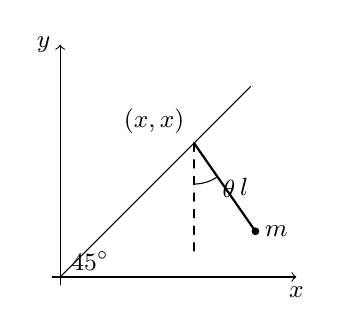
\begin{tikzpicture}[x=1cm,y=1cm,line cap=round,line join=round,font=\small]
  \draw[->] (-0.10,0) -- (3.00,0) node[below] {$x$};
  \draw[->] (0,-0.10) -- (0,2.95) node[left] {$y$};
  \draw[thin] (0,0) -- (2.42,2.42);
  \node at (0.38,0.20) {$45^\circ$};
  \coordinate (P) at (1.70,1.70);
  \coordinate (Q) at (2.48,0.58);
  \draw[dashed] (P) -- ++(0,-1.45);
  \draw[line width=0.8pt] (P) -- (Q);
  \fill (Q) circle (1.4pt);
  \node[above left] at (P) {$(x,x)$};
  \node[right] at (Q) {$m$};
  \node[right] at (2.16,1.14) {$l$};
  \draw (1.70,1.18) arc[start angle=-90,end angle=-55,radius=0.52];
  \node[right] at (1.94,1.12) {$\theta$};
\end{tikzpicture}

{\small 题 3 示意图}
\end{center}

\begin{enumerate}
  \item 写出拉格朗日量，并求出运动方程，要求写成
  \[
    \ddot\theta+f(\theta,x,\dot\theta,\dot x)=0,
    \qquad
    \ddot x+g(\theta,x,\dot\theta,\dot x)=0
  \]
  的形式；
  \item 写出广义动量，并写出哈密顿量。
\end{enumerate}

\begin{solution}
摆锤坐标为
\[
  X=x+l\sin\theta,
  \qquad
  Y=x-l\cos\theta .
\]
故
\[
  T=\frac12m\left[2\dot x^2+2l(\cos\theta+\sin\theta)\dot x\dot\theta
  +l^2\dot\theta^2\right],
\]
\[
  V=mg(x-l\cos\theta).
\]
于是
\[
  L=T-V.
\]
\begin{enumerate}
  \item 拉格朗日方程为
  \[
    2\ddot x+l(\cos\theta+\sin\theta)\ddot\theta
    +l(\cos\theta-\sin\theta)\dot\theta^2+g=0,
  \]
  \[
    l\ddot\theta+(\cos\theta+\sin\theta)\ddot x+g\sin\theta=0.
  \]
  这两式可联立解出
  \[
    \ddot\theta+f(\theta,x,\dot\theta,\dot x)=0,
    \qquad
    \ddot x+g_1(\theta,x,\dot\theta,\dot x)=0.
  \]
  其中右端实际上不显含 $x$ 和 $\dot x$。
  \item 广义动量为
  \[
    p_x=2m\dot x+ml(\cos\theta+\sin\theta)\dot\theta,
  \]
  \[
    p_\theta=ml(\cos\theta+\sin\theta)\dot x+ml^2\dot\theta .
  \]
  记 $D=\cos\theta+\sin\theta$，则哈密顿量为
  \[
    H=\frac{l^2p_x^2-2lDp_xp_\theta+2p_\theta^2}
    {2ml^2(2-D^2)}+mg(x-l\cos\theta).
  \]
\end{enumerate}


\medskip
\textbf{小问 (1) 的显式形式：}题目要求写成 $\ddot\theta+f=0$、$\ddot x+g=0$，可把两条方程看作关于 $\ddot x,\ddot\theta$ 的线性方程组。记
\[
  D=\cos\theta+\sin\theta,
  \qquad C=\cos\theta-\sin\theta,
\]
则
\[
  \begin{pmatrix}2&lD\\D&l\end{pmatrix}
  \begin{pmatrix}\ddot x\\\ddot\theta\end{pmatrix}
  =\begin{pmatrix}-lC\dot\theta^2-g\\-g\sin\theta\end{pmatrix}.
\]
行列式为
\[
  l(2-D^2)=l(1-\sin2\theta),
\]
在非奇异构型下得到
\[
  \ddot x=\frac{-lC\dot\theta^2-g+lDg\sin\theta}{2-D^2},
\]
\[
  \ddot\theta=\frac{D(lC\dot\theta^2+g)-2g\sin\theta}{l(2-D^2)}.
\]
因此可取
\[
  f=-\ddot\theta,
  \qquad g_1=-\ddot x,
\]
这也说明方程不显含 $x$，但势能中有 $mgx$，所以 $x$ 本身不是循环坐标。
\end{solution}
\end{question}

\begin{question}[铰接细棒的稳定性]
两根细棒用铰链连接，只能在同一平面内转动。其中一根细棒的质量为 $m$、长度为 $l$；另一根细棒始终竖直，并绕自身轴线以恒定角速度 $\Omega$ 转动。考虑重力作用：
\begin{enumerate}
  \item 写出系统的拉格朗日量，并求运动方程；
  \item 讨论系统的稳定性。
\end{enumerate}

\begin{solution}
设有质量的细杆与竖直向下方向夹角为 $\theta$。由于另一根竖直杆以角速度 $\Omega$ 绕竖直轴转动，有质量细杆所在的竖直平面也以同样角速度转动。距铰链 $s$ 处的质元速度平方为
\[
  v^2=s^2\dot\theta^2+\Omega^2s^2\sin^2\theta .
\]
积分 $\int_0^l s^2(m/l)\dd s=ml^2/3$，得
\[
  T=\frac16ml^2\left(\dot\theta^2+\Omega^2\sin^2\theta\right),
  \qquad
  V=-\frac12mgl\cos\theta .
\]
因此
\[
  L=\frac16ml^2\dot\theta^2+\frac16ml^2\Omega^2\sin^2\theta
  +\frac12mgl\cos\theta .
\]
\begin{enumerate}
  \item Euler--Lagrange 方程为
  \[
    \frac13ml^2\ddot\theta
    -\left(\frac13ml^2\Omega^2\sin\theta\cos\theta
    -\frac12mgl\sin\theta\right)=0,
  \]
  即
  \ansmath{\ddot\theta+\biggl(\frac{3g}{2l}-\Omega^2\cos\theta\biggr)\sin\theta=0.}
  \item 竖直向下位置 $\theta=0$ 附近，线性化方程为
  \[
    \ddot\theta+\left(\frac{3g}{2l}-\Omega^2\right)\theta=0.
  \]
  因此
  \ansmath{\Omega^2<\frac{3g}{2l}}
  时竖直向下平衡稳定，小振动角频率为
  \[
    \omega_s=\sqrt{\frac{3g}{2l}-\Omega^2}.
  \]
  当 $\Omega^2>3g/(2l)$ 时，$\theta=0$ 失稳，并出现非零平衡角
  \[
    \cos\theta_0=\frac{3g}{2l\Omega^2}.
  \]
  这些非零平衡是稳定的，因为等效势在该处取局部极小。临界情形 $\Omega^2=3g/(2l)$ 需要保留高阶项判断。
\end{enumerate}
\end{solution}

\end{question}

\begin{question}[一维谐振子的 Hamilton--Jacobi 解]
用 Hamilton--Jacobi 方程求解一维谐振子。为简单起见，设
\[
  H=\frac12\left(p^2+x^2\right).
\]

\begin{solution}
Hamilton--Jacobi 方程为
\[
  \frac{\partial S}{\partial t}
  +\frac12\left[\left(\frac{\partial S}{\partial x}\right)^2+x^2\right]=0.
\]
令
\[
  S=W(x,E)-Et,
\]
则
\[
  \left(\frac{\dd W}{\dd x}\right)^2+x^2=2E.
\]
因此
\[
  W=\int \sqrt{2E-x^2}\,\dd x
  =\frac{x}{2}\sqrt{2E-x^2}+E\arcsin\frac{x}{\sqrt{2E}}.
\]
由
\[
  \frac{\partial S}{\partial E}=\beta
\]
得
\[
  \arcsin\frac{x}{\sqrt{2E}}-t=\beta .
\]
故
\[
  \boxed{x(t)=\sqrt{2E}\sin(t+\beta)},
  \qquad
  \boxed{p(t)=\sqrt{2E}\cos(t+\beta)}.
\]


\medskip
\textbf{关键步骤：}这里分离常数 $E$ 就是系统能量。由
\[
  p=\frac{\partial S}{\partial x}=\sqrt{2E-x^2}
\]
可知运动被限制在 $|x|\le\sqrt{2E}$。第二个积分常数由
\[
  \frac{\partial S}{\partial E}=\beta
\]
给出，它本质上是初相位。若写成
\[
  x=\sqrt{2E}\sin(t+\beta),
\]
则
\[
  p=\dot x=\sqrt{2E}\cos(t+\beta),
\]
并且
\[
  H=\frac12(p^2+x^2)=E.
\]
这一步完成了从 Hamilton--Jacobi 完全积分到实际轨道的还原。


\medskip
Hamilton--Jacobi 方法给出的 $S=W-Et$ 实际上产生了到新常数变量的正则变换。若取新动量为 $P=E$，则新坐标为
\[
  Q=\frac{\partial S}{\partial P}=\frac{\partial W}{\partial E}-t.
\]
由于变换后新哈密顿量为零，$P,Q$ 均为常数。把 $Q=\beta$ 反解为 $x(t)$，就是完整求解。若进一步引入作用量
\[
  I=\frac{1}{2\pi}\oint p\,\dd x=E,
\]
则角变量为 $w=t+\beta$，这与谐振子频率为 $1$ 完全一致。
\end{solution}
\end{question}

\begin{question}[转动圆环上的滑块]
如图，半径为 $R$ 的圆环上有一个质量为 $m$ 的滑块。圆环可绕竖直直径转动，其转动惯量为 $I$。初始时，滑块位于圆环最上端，圆环的角速度为 $\omega_0$。此后滑块受到微扰而离开初始位置。设滑块与圆心连线和竖直方向的夹角为 $\theta$。

\begin{center}
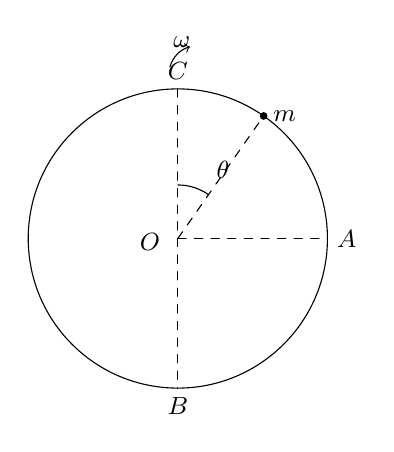
\begin{tikzpicture}[x=1cm,y=1cm,line cap=round,line join=round,font=\small]
  \draw[thin] (0,0) circle (1.90);
  \draw[dashed] (0,1.90) -- (0,-1.90);
  \draw[dashed] (0,0) -- (1.90,0);
  \coordinate (O) at (0,0);
  \coordinate (C) at (0,1.90);
  \coordinate (B) at (0,-1.90);
  \coordinate (A) at (1.90,0);
  \coordinate (M) at ({1.90*cos(55)},{1.90*sin(55)});
  \draw[dashed] (O) -- (M);
  \fill (M) circle (1.4pt);
  \node[above] at (C) {$C$};
  \node[right] at (A) {$A$};
  \node[below] at (B) {$B$};
  \node[left] at (-0.10,-0.04) {$O$};
  \node[right] at (M) {$m$};
  \draw[->] (-0.10,2.18) arc[start angle=165,end angle=105,radius=0.36];
  \node[above] at (0.05,2.30) {$\omega$};
  \draw (0,0.68) arc[start angle=90,end angle=55,radius=0.68];
  \node[right] at (0.37,0.87) {$\theta$};
\end{tikzpicture}

{\small 题 6 示意图}
\end{center}

\begin{enumerate}
  \item 给出系统的哈密顿量以及正则方程；
  \item 写出系统的初积分，并求出滑块到达 $A$、$B$ 两点时滑块的速度与圆环的角速度。
\end{enumerate}

\begin{solution}
取质点相对竖直向上方向的夹角为 $\theta$，圆环绕竖直轴的转角为 $\varphi$。质点到转轴的距离为 $R\sin\theta$，故
\[
  T=\frac12mR^2\dot\theta^2
  +\frac12\left(I+mR^2\sin^2\theta\right)\dot\varphi^2,
  \qquad
  V=mgR\cos\theta .
\]
正则动量为
\[
  p_\theta=mR^2\dot\theta,
  \qquad
  p_\varphi=\left(I+mR^2\sin^2\theta\right)\dot\varphi .
\]
\begin{enumerate}
  \item 哈密顿量为
  \ansmath{H=\frac{p_\theta^2}{2mR^2}
    +\frac{p_\varphi^2}{2\left(I+mR^2\sin^2\theta\right)}+mgR\cos\theta.}
  哈密顿正则方程为
  \[
    \dot\theta=\frac{p_\theta}{mR^2},
    \qquad
    \dot\varphi=\frac{p_\varphi}{I+mR^2\sin^2\theta},
  \]
  \[
    \dot p_\theta=\frac{p_\varphi^2mR^2\sin\theta\cos\theta}
    {(I+mR^2\sin^2\theta)^2}+mgR\sin\theta,
    \qquad
    \dot p_\varphi=0 .
  \]
  \item 两个初积分是
  \ansmath{p_\varphi=\text{const.},\qquad H=\text{const.}}
  初始条件为 $\theta=0$、$\dot\theta=0$、$\dot\varphi=\omega_0$，所以
  \[
    p_\varphi=I\omega_0,
    \qquad
    H=\frac12I\omega_0^2+mgR .
  \]
  到达侧点 $B$ 时 $\theta=\pi/2$，有
  \ansmath{\dot\varphi_B=\frac{I\omega_0}{I+mR^2}.}
  沿圆环切向的相对速度 $u_B=R|\dot\theta_B|$ 满足
  \[
    \frac12m u_B^2
    =mgR+\frac12I\omega_0^2-\frac12\frac{I^2\omega_0^2}{I+mR^2},
  \]
  即
  \ansmath{u_B=\sqrt{2gR+\frac{IR^2\omega_0^2}{I+mR^2}}.}
  质点在惯性系中的总速度还包含绕竖直轴的分量 $R\dot\varphi_B$，因此
  \[
    v_{B,\mathrm{inertial}}^2
    =u_B^2+R^2\dot\varphi_B^2 .
  \]
  到达最低点 $C$ 时 $\theta=\pi$，质点到转轴距离为零，因此
  \ansmath{\dot\varphi_C=\omega_0,\qquad u_C=v_{C,\mathrm{inertial}}=2\sqrt{gR}.}
\end{enumerate}
\end{solution}

\end{question}

\begin{question}[泊松括号与运动积分]
若物理量 $f(p_\alpha,q_\alpha,t)$ 满足 $\dd f/\dd t=0$，则称 $f$ 为运动积分。已知 $f(p_\alpha,q_\alpha,t)$ 和 $g(p_\alpha,q_\alpha,t)$ 是两个不显含时间的运动积分，证明它们的泊松括号 $[f,g]$ 也是运动积分。

\begin{solution}
因为 $f$ 和 $g$ 均不显含时间，且都是运动积分，故
\[
  \frac{\dd f}{\dd t}=\{f,H\}=0,
  \qquad
  \frac{\dd g}{\dd t}=\{g,H\}=0.
\]
利用 Jacobi 恒等式，
\[
  \{\{f,g\},H\}+\{\{g,H\},f\}+\{\{H,f\},g\}=0.
\]
后两项为零，因此
\[
  \{\{f,g\},H\}=0.
\]
又因为 $f,g$ 不显含时间，$\{f,g\}$ 也不显含时间，所以
\[
  \frac{\dd}{\dd t}\{f,g\}=\{\{f,g\},H\}=0.
\]
故泊松括号 $\{f,g\}$ 也是运动积分。这就是泊松定理的直接应用。


\medskip
\textbf{关键步骤：}泊松括号定义为
\[
  \{f,g\}=\sum_\alpha\left(
  \frac{\partial f}{\partial q_\alpha}\frac{\partial g}{\partial p_\alpha}
  -\frac{\partial f}{\partial p_\alpha}\frac{\partial g}{\partial q_\alpha}
  \right).
\]
对任一不显含时间的物理量 $A$，沿 Hamilton 流的全导数为
\[
  \frac{\dd A}{\dd t}=\{A,H\}.
\]
因此本题的关键不是直接展开所有偏导数，而是使用 Jacobi 恒等式。若 $f$ 或 $g$ 显含时间，则还必须额外保留 $\partial f/\partial t$、$\partial g/\partial t$，结论需要相应修正；题目中特别说明“不含时”正是为了避免这一项。


\medskip
也可以把证明写成一行算符形式。设 $D_t A=\partial A/\partial t+\{A,H\}$。本题中 $\partial f/\partial t=\partial g/\partial t=0$ 且 $D_tf=D_tg=0$。于是
\[
  D_t\{f,g\}=\{D_tf,g\}+\{f,D_tg\}=0,
\]
其中等号背后正是泊松括号满足 Jacobi 恒等式。这个写法强调了 Hamilton 流保持泊松结构，因此运动积分在泊松括号下封闭。
\end{solution}
\end{question}

\begin{question}[薛定谔场的拉格朗日量密度]
已知拉格朗日量密度
\[
  \mathcal{L}
  =-\frac{\hbar^2}{2m}\nabla\psi^*\cdot\nabla\psi
   -V\psi^*\psi+\ii\hbar\psi^*\dot\psi.
\]
将 $\psi$ 和 $\psi^*$ 视为独立场变量：
\begin{enumerate}
  \item 用修正的 Hamilton 原理导出 $\psi$ 和 $\psi^*$ 的运动方程；
  \item 求对应的正则动量密度以及哈密顿量密度。
\end{enumerate}

\begin{solution}
把 $\psi$ 和 $\psi^*$ 视为独立场变量。拉格朗日量密度为
\[
  \mathcal L=-\frac{\hbar^2}{2m}\nabla\psi^*\cdot\nabla\psi
  -V\psi^*\psi+\ii\hbar\psi^*\dot\psi .
\]
\begin{enumerate}
  \item 对 $\psi^*$ 变分，有
  \[
    \frac{\partial\mathcal L}{\partial\psi^*}
    =-V\psi+\ii\hbar\dot\psi,
    \qquad
    \frac{\partial\mathcal L}{\partial(\nabla\psi^*)}
    =-\frac{\hbar^2}{2m}\nabla\psi .
  \]
  Euler--Lagrange 方程给出
  \[
    -V\psi+\ii\hbar\dot\psi
    +\frac{\hbar^2}{2m}\nabla^2\psi=0,
  \]
  即
  \ansmath{\ii\hbar\frac{\partial\psi}{\partial t}
    =-\frac{\hbar^2}{2m}\nabla^2\psi+V\psi.}
  对 $\psi$ 变分则得复共轭方程
  \ansmath{-\ii\hbar\frac{\partial\psi^*}{\partial t}
    =-\frac{\hbar^2}{2m}\nabla^2\psi^*+V\psi^*.}
  \item 正则动量密度为
  \[
    \pi_\psi=\frac{\partial\mathcal L}{\partial\dot\psi}=\ii\hbar\psi^*,
    \qquad
    \pi_{\psi^*}=\frac{\partial\mathcal L}{\partial\dot\psi^*}=0.
  \]
  第二个等式是一次时间导数场论的约束，说明该拉格朗日量是奇异的。哈密顿量密度由 Legendre 变换得
  \[
    \mathcal H=\pi_\psi\dot\psi+\pi_{\psi^*}\dot\psi^*-\mathcal L
    =\frac{\hbar^2}{2m}\nabla\psi^*\cdot\nabla\psi+V\psi^*\psi .
  \]
  因此
  \ansmath{\mathcal H=\frac{\hbar^2}{2m}|\nabla\psi|^2+V|\psi|^2.}
\end{enumerate}


\medskip
\textbf{边界项处理：}对场变量变分时，需要对空间梯度项分部积分。例如
\[
  \delta\int \nabla\psi^*\cdot\nabla\psi\,\dd^3x
  =-\int \delta\psi^*\nabla^2\psi\,\dd^3x
\]
其中边界变分取零。由于拉氏密度只含 $\dot\psi$ 而不含 $\dot\psi^*$，所以 $\pi_{\psi^*}=0$ 是初级约束；这并不影响由 Euler--Lagrange 方程得到薛定谔方程，但在严格 Hamilton 场论中需要作为约束处理。
\end{solution}

\end{question}
